\chapter{Modelling swarming systems}
\label{chapter:swarming_systems}
With swarming systems, we indicate the class of all processes of collective motion. From the most specific processes, which are for example the dynamics in a flock of birds, a school of fish or the behaviour of a crowd of people, to the most general processes, such as collective motion in systems of self-propelled particles, which obey certain prescribed interaction rules. The process of self-organisation in such systems is still poorly understood. So far, research into swarming systems was mainly done in either of two ways. The swarm was represented as a continuous medium \cite{Toner1998}, or (comprehensive) agent-based models were developed that obey certain dynamical rules \cite{Huepe2011, VanDrongelen2015, Vicsek1995, Vicsek2012}. Since a few years, research into the application of adaptive networks on swarming systems has gotten more attention \cite{Huepe2011, Chen2016, Zschaler2012}. In the next section, we will apply the developed continuous state adaptive network model to a swarming system.

The most famous minimal agent-based model of collective motion is the Vicsek model \cite{Vicsek1995}. It describes a system of self-propelled individuals moving at a constant speed $v$. These individuals try to align with all their neighbours within a certain radius $r$, such that the system can be (discretely) evolved as 
\begin{subequations}
\begin{alignat}{2}
	\bm{x_i}(t+\Delta t) &= \bm{x}_i(t) + \bm{v}_i \Delta t\\
	\theta_i(t+\Delta t) &= \langle \theta_j \rangle_{|r_i - r_j | <r} + \eta_i
\end{alignat}
\end{subequations}
in which $\bm{x_i}(t)$ represents the position of the $i$'th individual at time $t$. The direction of its velocity is given by $\theta_i(t)$. $\eta_i$ is a noise parameter, which can for example be drawn from a uniform probability distribution on the interval $(-\pi,\pi]$.

Although many great advances have been made with (variations on) the Vicsek model \cite{Vicsek2012}, there is a restriction on the size of the system. The position and direction of each individual should be updated each time step, which may lead to computationally heavy simulations. For adaptive networks, there is no such limit. The accuracy even improves for increasing system size, such that these models allow for obtaining more general results. Therefore, modelling swarming systems in an adaptive network might give new insights into the self-organisation in large swarming systems. 


\section{Applying the developed adaptive network models to swarming systems}
\label{section:applying_network_to_swarming}
So far, the adaptive network models have been derived in the most general form possible. In the last part of this thesis, we will apply them to swarming systems of two-dimensional motion. All individuals are represented by a node and individuals that are aware of each other's behaviour are connected by a link. This allows for a very similar condition to the alignment in the Vicsek model, where individuals tend to align with their neighbours within a certain radius. We will refer to individuals connected by a link as neighbours. Moreover, we assume that all individuals can be modelled as self-propelled particles with a constant speed $v$, such that only their direction of movement is of importance. In this work, we will restrict the individuals to move in two dimensions only. Hence, it would be a sensible choice to define $\Omega = (-\pi,\pi]$. Furthermore, we can make the four types of interactions more specific:

\begin{description}
	\item [Type 1] Individuals pick another direction with rate $\eta$. This direction is uniformly chosen from $\Omega = (-\pi,\pi]$
	\item [Type 2] Individuals adopt to the average direction of two neighbours with rate $\sigma_c$.
	\item [Type 3] Arbitrarily chosen not-neighbouring individuals become neighbours with rate $\alpha$.
	\item [Type 4] Arbitrarily chosen neighbours become not-neighbouring individuals with rate $\beta$.
\end{description}

All dynamics take place irrespective of any additional neighbours an individual may have. A swarming system can be well described with these four types of interactions. The first two types are comparable to the Vicsek model; type 1 is similar to the noise $\eta_i$ of the $i$'th particle, whereas type 2 corresponds to the tendency of individuals to align with their neighbours within a certain radius. This radius is in the network modelled with the links since we do not keep track of the physical position of individuals in space. Interactions of the third type are needed since not-neighbouring individuals which move in different directions might become aware of each other's position at a certain moment. It is sufficient to model this by a global rate because we do not look at individual nodes separately (which would also not be possible since we do not know the individuals' physical position). The main advantage here is that this allows for faster computations. The fourth type of dynamics is the opposite of the third type; individuals which are neighbouring, but head in different directions are at a certain moment too far apart to be still aware of each other. Therefore their link must be broken. Again, it is sufficient to model this with a global rate. 

In this case, the meaning of the state distribution function $f(x;t)$ can be explained as follows: the network density of individuals with direction $x$ in the interval $[\theta_1,\theta_2]$ at time $t$ is given by 
\[
\int\limits_{\theta_1}^{\theta_2} d\bar{x}\ f(\bar{x};t).
\]
For the link distribution function $l(x,y;t)$ we have something similar: the density of pairs of neighbouring individuals, where one of the neighbours' direction $x$ is within the interval $[\theta_1,\theta_2]$, while the other heads in a direction $y$ in the interval $[\phi_1,\phi_2]$, at time $t$, is given by 
\[
\int\limits_{\theta_1}^{\theta_2} d\bar{x}\ \int\limits_{\phi_1}^{\phi_2} d\bar{y}\ l(\bar{x},\bar{y};t).
\]

So far, we have not mentioned how the averaging operation in the model is defined, because this definition can differ for various applications. This operation corresponds to the integrals over $\xi$ in \cref{eq:cont_complete}. In the case of two-dimensional motion, the average should be taken in a special way, because the interval is periodic. This is easiest illustrated in an example. Suppose one individual has a direction of $\theta_1=\frac{3\pi}{4}$, while another individual moves in the $\theta_2 = -\frac{3\pi}{4}$ direction. The numerical average would be zero, while the `angular' average is $\theta=\pi$. In this case, we clearly should use the latter. This can be implemented in the equations by integrating over $\xi$ from $0$ to $\frac{\pi}{2}$, instead of integrating over the complete state set $\Omega$.  \Cref{fig:cont_states_averaging_k} illustrates this process of finding the right states which average direction $x$. Every pair of individuals heading in directions $x-\xi$ and $x+\xi$ respectively have the possibility to let a common neighbour change its direction to $x$ as long as $\xi \in \left[0,\frac{\pi}{2}\right)$.


\begin{figure}[t]
	\centering
	\begin{tikzpicture}[rotate=30]
	\draw[thick] (0,0) coordinate(O) circle (3);
	\draw[dashed] (-3.2,0) node[left] {$x-\frac{\pi}{2}$} -- (3.2,0) node[right] {$x+\frac{\pi}{2}$};
	\draw (0,-3) coordinate(under) node[below,xshift=0.1cm] {$x$} -- (0,0); 
	\draw[rotate=35] (-3,0) coordinate(left) node[left, yshift=-0.2cm] {$x-\xi $} -- (0,0);
	\draw[rotate=-35] (0,0) -- (3,0) coordinate(right) node[right] {$x+\xi $};
	\draw pic["$\xi $", <-, draw, thick,angle radius=10mm] {angle = left--O--under};% node[xshift=0cm, yshift=-1.3cm] {$\xi $};
	\draw pic["$\xi $", ->, draw, thick,angle radius=12mm] {angle = under--O--right};% node[xshift=1.25cm, yshift=-0.85cm] {$\xi $};
	\end{tikzpicture}
	\caption{The process of finding the right directions $x-\xi $ and $x+\xi $ which average to $x$. Clearly $\xi \in \left[0,\frac{\pi}{2}\right)$ or the average will be in the direction $x+\pi$.}
	\label{fig:cont_states_averaging_k}
\end{figure}

Now we have all variables, functions and dynamics rules properly defined to apply the previously derived network to swarming systems. In the next two sections, the resulting sets of equations for both the mean field approximation and the moment closure approximation models are stated, including results and corresponding analysis.

\section{Mean field approximation on swarming systems}
All rules making the continuous state adaptive network model a swarming system were described in the previous section. In this section, they will be applied to the mean field approximation. Subsequently, analysis and discussion of the results will follow. 

The partial differential \cref{eq:cont_state_mean_field} models the collective motion in the previously described swarm if we write it as 

\begin{equation}
\begin{aligned}
\frac{\partial}{\partial t}\ f(x;t) =\ & 
\eta \left( \frac{1}{2\pi} - f(x;t) \right) \\
&	+ \sigma_c\langle k \rangle^2  \int\limits_{0}^{\pi/2} d\xi\
f(x-\xi;t)\ f(x+\xi;t) \\
&	- \sigma_c \langle k \rangle^2\ f(x;t) \int\limits_{-\pi}^\pi dz \int\limits_{0}^{\pi/2} d\xi\ f(z-\xi;t)\ f(z+\xi;t).
\label{eq:cont_state_mean_field_swarming}
\end{aligned}
\end{equation}


\subsection{Discretisation}
It is unlikely that we can find the time-dependent solution to this equation analytically, consequently let us look for a numerical solution. The first step will be discretising the time and state set $\Omega$. This will yield a partial \textit{difference} equation which can be solved using a computer.
The continuous time $t = [0, T_{\text{max}}]$ at which the network evolution is considered will be partitioned into $M$ intervals of length $\Delta t$, such that the discrete time set is of the form 
\[ t_d= \{0, \Delta t, 2 \Delta t, ... , (\tau-1) \Delta t,  \tau\Delta t, ..., T_{\text{max}} - \Delta t, T_{\text{max}}  \}, \]
in which $M \Delta t = T_{\text{max}}$ and $\tau$ is the discrete time index. Next, we have to discretise the state set $\Omega$. This set is partitioned into $N$ intervals of length $\Delta \omega$, such that $\Omega = (-\pi,\pi]$ is transformed into 
\[\Omega_d = \{-\pi, -\pi+\Delta\omega,...,-\pi+ (p-1) \Delta\omega, -\pi+ p \Delta\omega, ... \pi-\Delta\omega, \pi \}, \]
in which $N \Delta \omega = 2\pi$ and $p$ is the discrete state index.\footnote{It might seem odd to discretise the state set as we have just made it continuous. Ironically this is the first step in solving the system numerically. It is however important to note that the discretisation is different from the discrete state model. This discretisation gives the same solutions as the continuous state model would if it were solved analytically if we take the limits of $\Delta t \to 0$ and $\Delta \omega \to 0$. Moreover, it incorporates the different dynamics which are used exclusively in the continuous state case. In other words, we are really solving a different system.}
Furthermore, we use the following shorthand notation in the discretisation of the density function $f(x;t)$, 
\[
f_{p}^{\tau } = f(-\pi+p\Delta \omega; \tau \Delta t).
\]
The discrete state-time-grid which is obtained is visualised in \cref{fig:grid_pde}.

\begin{figure}[htp]
	\centering
	\begin{tikzpicture}[dot/.style={draw,circle,minimum size=0.6mm,inner sep=0pt,outer sep=0pt,fill=black}]
	\path \foreach \x/\y [count=\k from 0] in { 0/0,  1/0, 2/0, 3/0, 4/0, 5/0, 6/0, 7/0, 0/1,  1/1, 2/1, 3/1, 4/1, 5/1, 6/1, 7/1, 0/2,  1/2, 2/2, 3/2, 4/2, 5/2, 6/2, 7/2, 0/3,  1/3, 2/3, 3/3, 4/3, 5/3, 6/3, 7/3,0/4,  1/4, 2/4, 3/4, 4/4, 5/4,6/4, 7/4,0/5,  1/5, 2/5, 3/5, 4/5, 5/5,6/5,7/5, 0/6,1/6,2/6,3/6,4/6,5/6,6/6, 7/6}
	{coordinate [dot] (p\k) at (\x,\y)}; 
	
	\draw[->] (6.7,-0.5)--(7,-0.5) node[below] at (3.5,-1) {$t$};
	\draw[] (0,-0.5)--(0.3,-0.5);
	\draw[] (0.7,-0.5)--(6.3, -0.5);
	\draw[dotted] (0.3,-0.5)--(0.7,-0.5);
	\draw[dotted] (6.3,-0.5)--(6.7,-0.5);
	
	\draw[->] (-0.5,5.7)--(-0.5,6) node[left] at (-1.2,3) {$\Omega$};
	\draw[<-] (-0.5, 0)--(-0.5,0.3);
	\draw[] (-0.5,0.7)--(-0.5,5.3);
	\draw[dotted] (-0.5,0.3)--(-0.5,0.7);
	\draw[dotted] (-0.5,5.3)--(-0.5,5.7);
	
	\node[] at (0, -.75)  () {\small{$0$}}; 
	\node[] at (7, -.75)  () {\small{$T_{\text{max}}$}};
	\node[] at (-0.85, 0)  () {\small{$-\pi$}}; 
	\node[] at (-0.85, 6)  () {\small{$\phantom{-} \pi$}};
	\node[] at (-0.75, 3)  () {\small{$0$}};
	
	\node[] at (-1.15, 2)  () {\tiny{$-\pi + p \Delta \omega$}}; 
	\node[] at (4, -.75)  () {\tiny{$\tau \Delta t$}}; 
	\node[] at (4.25, 2.25)  () {\small{$f_{p}^{\tau}$}};
	
	\draw[<->] (1,1.05)--(1,1.95) node[left] at (1,1.5) {\small{$\Delta \omega$}};
	\draw[<->] (1.05,1)--(1.95,1) node[below] at (1.5,1) {\small{$\Delta t$}};
	\end{tikzpicture}
	\caption{Grid resulting from the discretisation of $t$ and $\Omega$. The time is discretised into $M$ time steps of size $\Delta t = \frac{T_\text{max}}{M}$ with corresponding index $\tau$. The state set $\Omega$ is discretised into $N$ discrete state values, with step size $\Delta \omega = \frac{2\pi}{N}$. The corresponding index is $p$.}
	\label{fig:grid_pde}
\end{figure}

The next step is discretising the partial differential equation. For the partial derivatives the forward difference method is applied. That is 
\begin{equation}
\label{eq:forward_difference_f}
\frac{\partial}{\partial t}\ f(x;t) \approx \frac{f(x;t+\Delta t) - f(x;t)}{\Delta t} = \frac{f_{p}^{\tau+1} - f_{p}^{\tau}}{\Delta t},
\end{equation}
for $x = -\pi + p \Delta \omega$. In addition, the integrals should be discretised. This can be done by replacing them by their corresponding left Riemann sum, such that
\begin{equation}
\label{eq:left_riemann}
\int\limits_{-\pi}^\pi dx\ f(x;t) \approx \Delta \omega  \sum\limits_{i=0}^{N-1}  f(\pi + i \Delta \omega;t) = \Delta \omega \sum\limits_{i=0}^{N-1}  f_{i}^{\tau}.
\end{equation}
Note, since the discretisation is done as a \textit{left} Riemann sum, the summation limits go from $i=0$ to $i=N-1$. Applying these discretisation steps to the partial differential equation yields a partial \textit{difference} equation. With that, the system in mean field approximation can be solved by a forward Euler scheme
\begin{equation}
\begin{aligned}
f_p^{\tau+1} &= 
f_p^\tau +
\Delta t \left[ \frac{\eta\ }{2 \pi} -\eta\ f_p^\tau 
+ \Delta \xi\, \sigma_c\ \langle k \rangle^2  \sum\limits_{i=0}^{\frac{N}{4}-1}\ \left( f_{p-i} ^\tau\ f_{p+i}^\tau
- \Delta z\ f_p^\tau \sum\limits_{j=0}^{N-1} f_{j-i}^\tau\ f_{j+i}^\tau \right)  \right],
\end{aligned}
\label{eq:cont_mean_field_swarm_discrete}
\end{equation}
such that we can `walk forward' in time by implementation of \cref{eq:cont_mean_field_swarm_discrete} in any appropriate computing language, given a feasible initial condition. 
\clearpage

\subsection{Results and discussion}

The forward Euler scheme of \cref{eq:cont_mean_field_swarm_discrete} was implemented in Python. The input parameters of the script are the system parameters $\eta$, $\sigma_c$, $\langle k \rangle$, step size $\Delta t = \frac{1}{300}$, and grid spacing $\Delta \omega = \frac{\pi}{400}$. To generate results a renormalised standard normal distribution was chosen as initial condition, i.e. 
\begin{equation}
f(x;0) = \frac{A}{\sqrt{2\pi\sigma_f^2}} \exp{\left(-\frac{(x-\mu_f)^2}{2\sigma_f^2}\right)},
\label{eq:gaussian}
\end{equation}
where $\mu_f = 0$ is the mean, $\sigma_f^2=1$ is the variance of the distribution and $A$ is determined such that $\int\limits_{-\pi}^\pi dx\ f(x;0) = 1$. Similar to the discrete state case, it turns out that the final state distribution only depends on a ratio of system parameters. In this case this important ratio is $\frac{\eta}{\sigma_c\langle k \rangle^2}$. In \cref{fig:cont_mean_field_final_dist} the final distribution $f(x;M\Delta t)$ after $M = 3\cdot 10^5$ time steps $\Delta t$ is plotted for various values of $\frac{\eta}{\sigma_c\langle k \rangle^2}$, together with the initial condition. 

\begin{figure}[tbp]
	\centering
	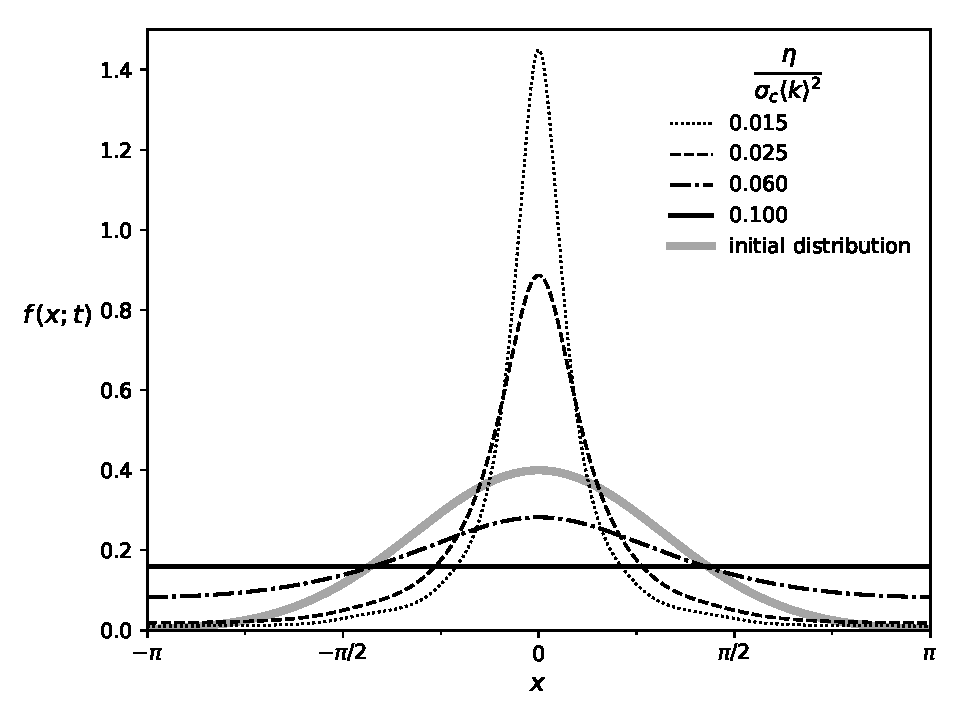
\includegraphics[width=0.7\linewidth]{figures/cont_mean_field_final_dist_BW}
	\caption{ The final state distribution $f(x;M\Delta t)$, for $M=3\cdot 10^5$ time steps, as a function of state $x$ for different values of the ratio $\frac{\eta}{\sigma_c\langle k \rangle^2}$ of system parameters. $M$ was large enough to ensure that the system converged to a stationary solution. The constant solution at $\frac{\eta}{\sigma_c\langle k \rangle^2} = 0.1$ is $f(x;t) = \frac{1}{2\pi}$. The system was initialised as a standard normal distribution (with zero mean and unit variance), however, note that the initial condition does not influence the outcome unless a stationary solution is chosen as initial condition.}
	\label{fig:cont_mean_field_final_dist}
\end{figure}

In order to verify that the final state distributions have converged (within certain numerical tolerance) to a stationary solution, the time evolution of the variance of the distribution $\sigma_f^2$ \footnote{Note that $\sigma_f^2$ is the variance of the state distribution $f(x;t)$ and $\sigma_c$ is the rate of three-body interactions.} is visualised in \cref{fig:cont_mean_field_var_vs_t}. After $\tau=300$ time steps, the variance has converged for almost all values of $\frac{\eta}{\sigma_c\langle k \rangle^2}$. In the situations where there was no convergence after 300 time steps, we verified that convergence of $\sigma_f^2$ was obtained at a later moment, before the end of the computation. If we combine this result with the fact that all feasible state distributions integrate to one on the state set $\Omega = (-\pi,\pi]$ and with the observation that the shape of the distribution remains the same in the last part of the simulation, we can conclude that the final distributions after $3\cdot 10^5$ time steps correspond to steady-state distributions. 

\begin{figure}[tbp]
	\centering
	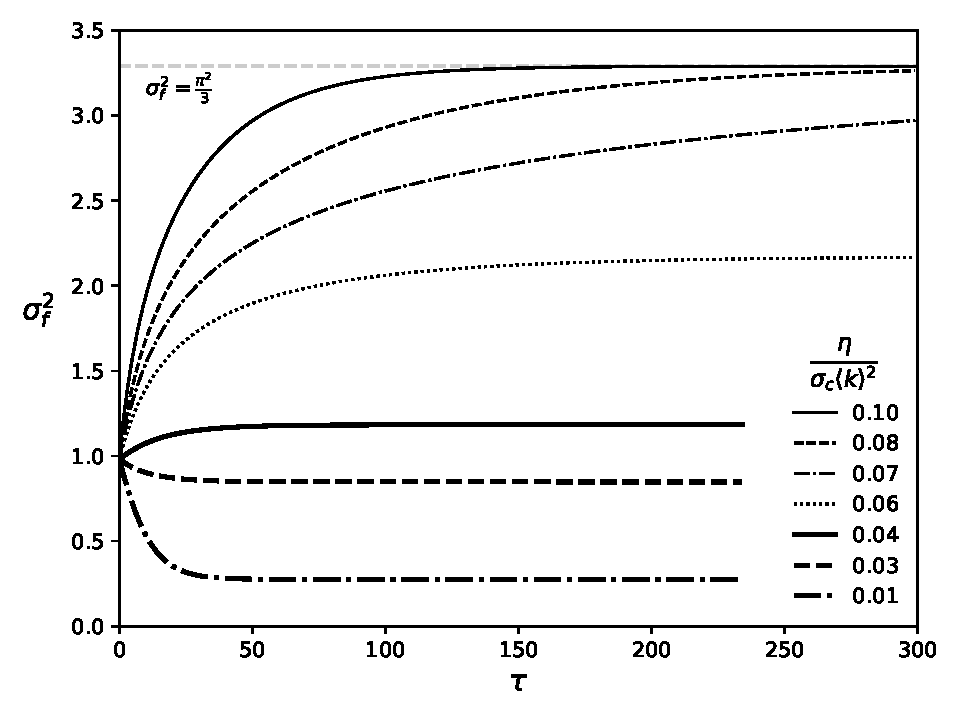
\includegraphics[width=0.7\linewidth]{figures/cont_mean_field_var_vs_t_BW}
	\caption{Time evolution of the variance $\sigma_f^2$ of the state distribution $f(x;t)$ for various values of $\frac{\eta}{\sigma_c\langle k \rangle^2}$. For almost all values of the system parameters convergence was achieved within 300 time steps. For $\frac{\eta}{\sigma_c\langle k \rangle^2} \in \{0.07, 0.08\}$ convergence was achieved at a later moment in the computation. $\sigma_f^2 = \frac{\pi^2}{3}$ corresponds to a uniform state distribution. The legend lists the curves from top to bottom. }
	\label{fig:cont_mean_field_var_vs_t}
\end{figure}

Comparing continuous state adaptive network models to the discrete state models, we have the following similarities. The disordered solution in which all possible states in $\Omega$ are equally distributed over all agents corresponds to the continuous uniform distribution. Furthermore, the ordered solution, in which there is one state occupied by a majority of nodes compared to all other states, is a bell-shaped distribution in the continuous case. In the limit to all nodes occupying the same state $f(x;t)$ becomes a Dirac delta distribution. In contrast to the discrete state networks, minority distributions do not have equal densities. We will use the variance of the distribution as a measure of the amount of order in the system. A system which is completely disordered is represented by a uniform distribution $f(x;t)=\frac{1}{2\pi}$, such that 
\begin{equation}
\sigma_f^2= \frac{1}{2\pi} \left[ \int\limits_{-\pi}^\pi dx\ x^2 - \left( \int\limits_{-\pi}^\pi dx\ x \right)^2 \right] = \frac{\pi^2}{3}.
\end{equation}
On the other hand, for a completely ordered system, which is represented by a Dirac delta distribution, we have $\sigma_f^2 \to 0$ by definition. Similar to the discrete state adaptive networks, the final state distribution depends on the ratio of system parameters. If there is a relatively high noise rate $\eta$, compared to $\sigma_c$ then the network tends to end up in a less ordered state compared to situations in which the rate $\sigma_c$ or the mean degree $\langle k \rangle$ is relatively high. In these latter cases, the system will evolve towards a more ordered distribution. We can make this quantitative by computing the variance of the stationary solution for multiple values of $\frac{\eta}{\sigma_c\langle k \rangle^2}$. The result is plotted in \cref{fig:cont_mean_field_variance_zoom}.

\begin{figure}[tbp]
	\centering
	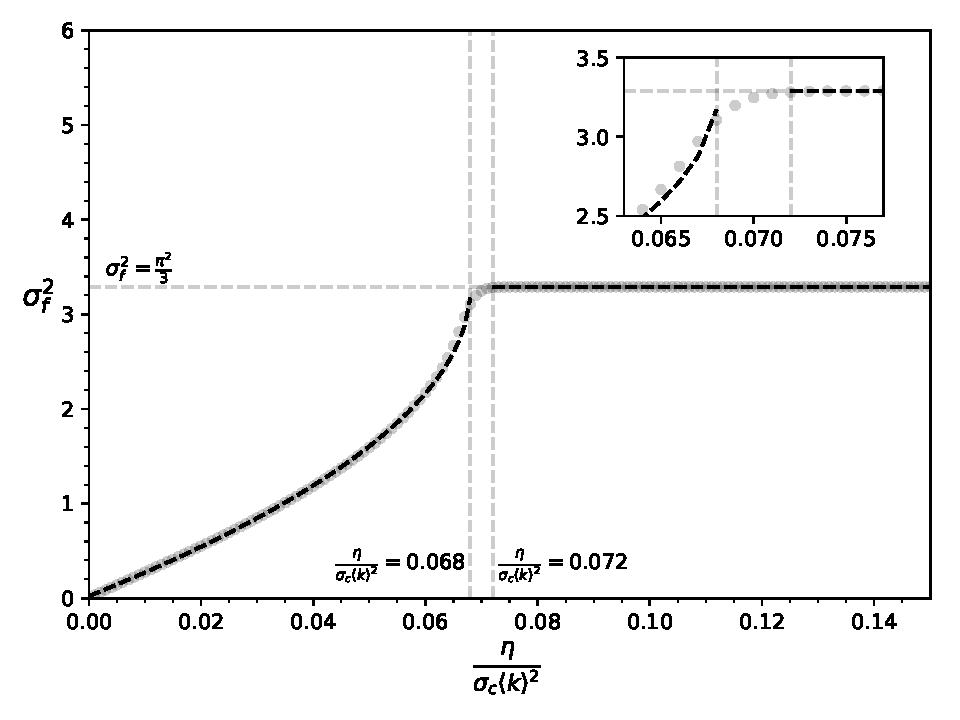
\includegraphics[width=0.7\linewidth]{figures/cont_mean_field_variance_zoom}
	\caption{Variance $\sigma_f^2$ of the stationary state of the state distribution $f(x;t)$ as function of the ratio $\frac{\eta}{\sigma_c\langle k \rangle^2}$ of mean field system parameters. The transition from a disordered to an ordered state occurs at $\frac{\eta}{\sigma_c\langle k \rangle^2} =0.068$. For $\frac{\eta}{\sigma_c\langle k \rangle^2} > 0.072$ the state distribution function is constant at $\frac{1}{2\pi}$ such that $\sigma_f=\frac{\pi^2}{3}$ and the system is completely disordered. For $\frac{\eta}{\sigma_c\langle k \rangle^2} < 0.068$ the state distribution has a maximum value for some state $x$, such that the system is ordered. On this interval, the black dashed line is a least squares fit of a square root function to all steady state variances $\sigma_f^2$. (Inset) A close up of the region in which the transition from the ordered to the disordered state occurs. The data points in this region do not fit the square root, nor the constant $\frac{\pi^2}{3}$. }
	\label{fig:cont_mean_field_variance_zoom}
\end{figure}

\begin{figure}[tbp]
	\centering
	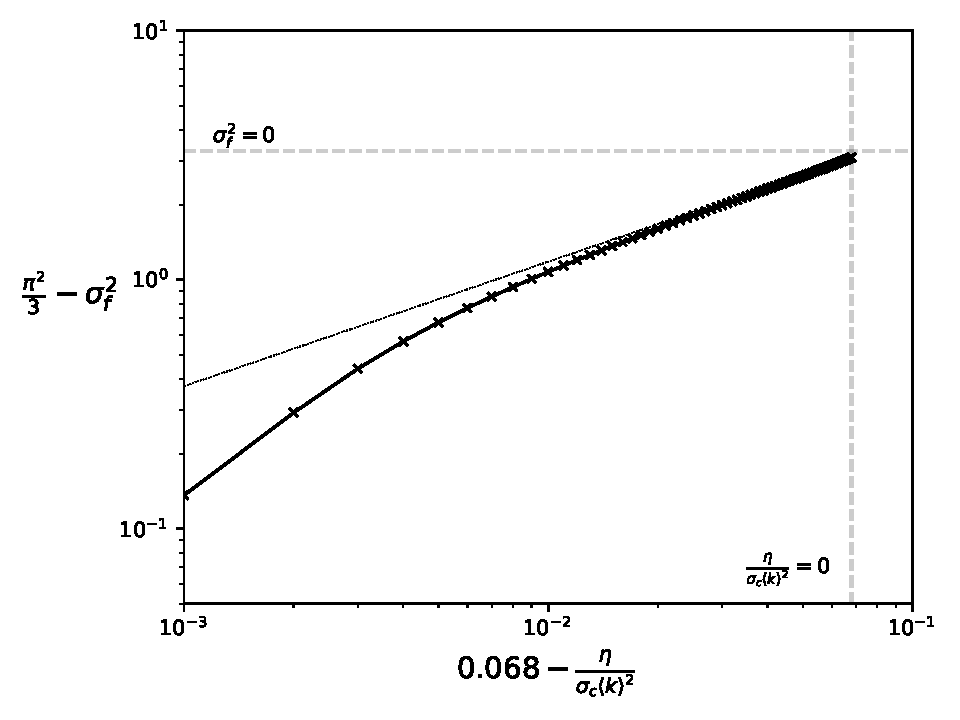
\includegraphics[width=0.7\linewidth]{figures/cont_mean_field_variance_loglog}
	\caption{Variance $\sigma_f^2$ of the stationary state of the state distribution $f(x;t)$ versus the ratio $\frac{\eta}{\sigma_c\langle k \rangle^2}$ of mean field system parameters on logarithmic scales. Only the ordered solutions $\left(\frac{\eta}{\sigma_c\langle k \rangle^2} < 0.068\right)$ were plotted. The dotted line has slope $\frac{1}{2}$, representing a square root function (with offset).}
	\label{fig:cont_mean_field_variance_loglog}
\end{figure}
\raggedbottom
For $\frac{\eta}{\sigma_c\langle k \rangle^2} > 0.072$ the variance $\sigma_f^2$ in the state distribution function $f(x;t)$ equals the expected variance for the disordered solution. For $\frac{\eta}{\sigma_c\langle k \rangle^2} < 0.068$ we have $\sigma_f^2 < \frac{\pi^2}{3}$, corresponding to a system in which one subset of states is more present than the others. These are the not-constant state distributions in \cref{fig:cont_mean_field_final_dist}. For discrete state networks, the density of a certain state as a function of the system parameters could be analytically expressed by a square root relationship \cite{Chen2016}. In order to check if a similar relation holds between the distribution variance and system parameters for the continuous state networks, the data points for $\frac{\eta}{\sigma_c\langle k \rangle^2} < 0.068$ are plotted on logarithmic scales in \cref{fig:cont_mean_field_variance_loglog}. Comparing the curve shape with the dotted square root function, we can see that especially for lower values of $\frac{\eta}{\sigma_c\langle k \rangle^2}$ the variances lie on a line with slope $\frac{1}{2}$, which is a property of a square root relation. Moreover, we can make a least squares fit of 
\begin{equation}
\sigma_f^2 = \frac{\pi^2}{3} - a \sqrt{0.068-\frac{\eta}{\sigma_c\langle k \rangle^2}}, \quad \text{for} \quad \frac{\eta}{\sigma_c\langle k \rangle^2} < 0.068, \qquad a \in \mathbb{R},
%[a,b]=[12.52327665,  0.0680888 ]
%np.pi**2/3 - a*np.sqrt(b - n)
%r2sqrt=  0.9991702860618208
\end{equation}
in \cref{fig:cont_mean_field_variance_zoom}. The optimal parameters is $a = 12.52$, with goodness of fit $R^2 = 0.999$. Hence we confirm that the relation is indeed given as a square root function. The variances for values $\frac{\eta}{\sigma_c\langle k \rangle^2} \in [0.068, 0.072]$ do not fit the least squares fit, nor the constant $\frac{\pi^2}{3}$. Hence, the transition from the ordered state to a disordered state occurs in this region. However, we can expect it to be closer to $0.068$, since this is where the fitted square root meets the variance of the disordered state. This is in line with the fact that systems with $\frac{\eta}{\sigma_c\langle k \rangle^2}$ close to the ratio at which the transition takes place tend to converge much slower than systems which have a much higher or lower ratio. This can also be observed in \cref{fig:cont_mean_field_var_vs_t}. It would mean that if we take both the simulation time and the number of grid points to infinity, we would have a perfect distinction between the disordered states on the branch where the variance is $\frac{\pi^2}{3}$ and the branch which can be described as a square root function. Taking everything together, the system ends up in an ordered state if $\frac{\eta}{\sigma_c\langle k \rangle^2} < 0.068$ and in a disordered state if $\frac{\eta}{\sigma_c\langle k \rangle^2}>0.068$, where convergence rates are very low for ratios close to $0.068$. 

Lastly, we check whether we can make a judicious guess for an analytic stationary solution which fits the simulation results. In the first place, it is not hard to see that 
\begin{equation}
f(x)=\frac{1}{2\pi}
\end{equation}
forms the disordered stationary solution.

One might expect the ordered state distribution to have a bell-shape. To check this, various final state distributions are plotted on a logarithmic scale versus the state $x$ on both linear and logarithmic scales in \cref{fig:cont_mean_field_linlog_loglog} to check if they can be represented by either renormalised Gaussian or renormalised Cauchy distributions. A Gaussian distribution is of the form
\begin{equation}
f(x; \mu_f, \sigma_f^2) = \frac{A}{\sqrt{2\pi\sigma_f^2}} \exp{\left(-\frac{(x-\mu_f)^2}{2\sigma_f^2}\right)},
\label{eq:gaussian_fit}
\end{equation}
in which $\mu_f$ represents the mean and $\sigma_f^2$ the variance of the distribution. This is an exponential function in $x^2$ and therefore it will appear as a parabola on a logarithmic-linear-plot. It is easy to see that the state distributions do not follow the shape of a parabola, from which we can conclude that the final distributions are not given as Gaussian distributions. The Cauchy distribution can be written as
\begin{equation}
f(x; x_0, \gamma) = \frac{A}{\pi \gamma} \frac{\gamma^2}{(x-x_0)^2+\gamma^2} 
\label{eq:cauchy_fit}
\end{equation}
with $A \in \mathbb{R}$ the amplitude, $x_0$ the location parameter, specifying the location of the maximum and $\gamma$ the scale parameter corresponding to the half-width at half-maximum. Supposing $x_0=0$, this distribution is a polynomial function in $x^2 + \gamma^2$, such that if it is plotted on a graph with logarithmic scales it will appear as a line with slope $-2$. \Cref{fig:cont_mean_field_linlog_loglog} shows that the final state distributions are very similar to Cauchy distributions, especially around $x=0$, the location of the peak of the distribution.
\begin{figure}[tbp]
	\centering
	\makebox[\textwidth][c]{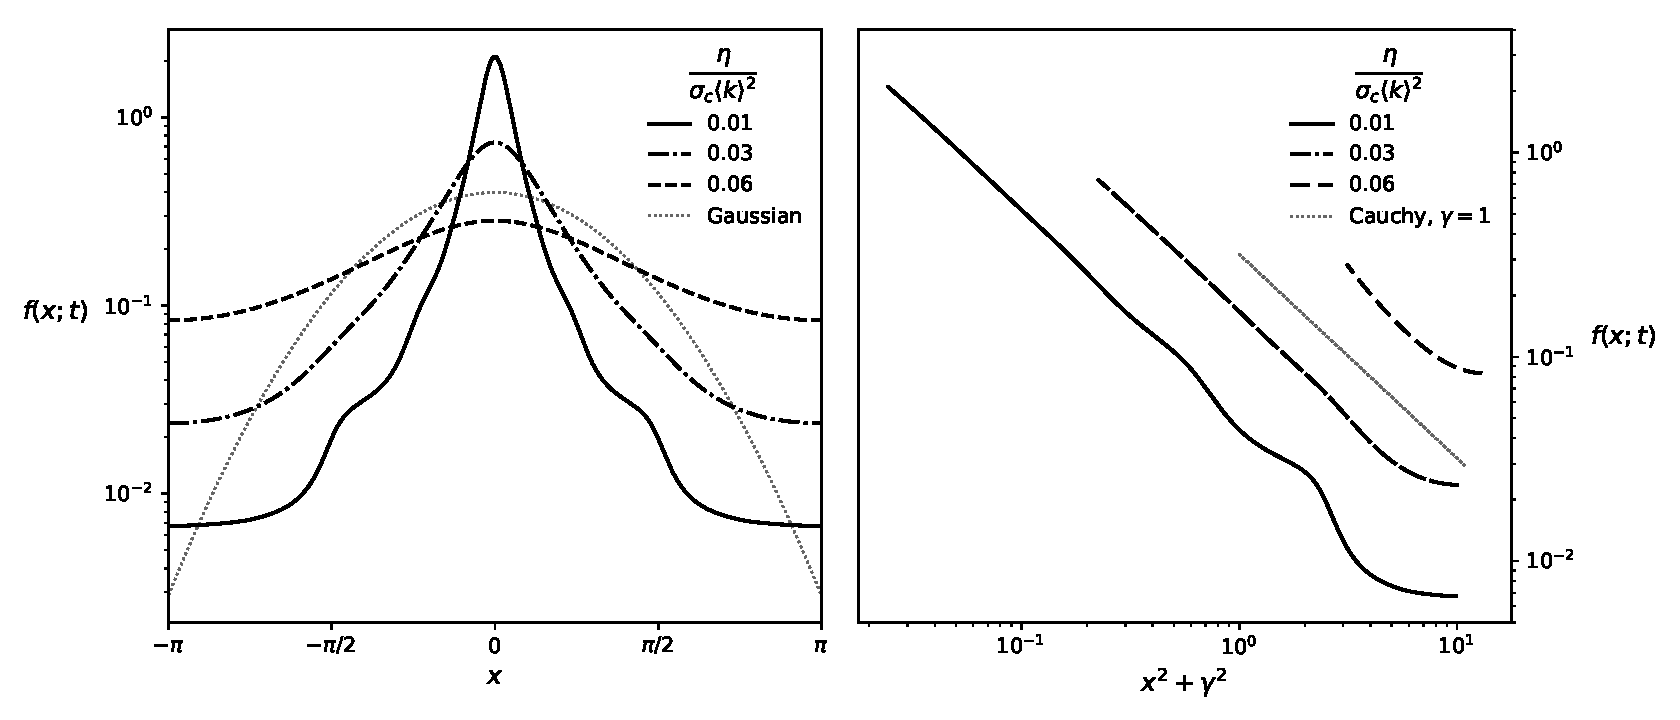
\includegraphics[width=1.2\linewidth]{figures/cont_mean_field_linlog_loglog}}%
	\caption{(left) The final state distribution function $f(x,M\Delta t)$ for $M=3\cdot 10^5$, for various values of $\frac{\eta}{\sigma_c\langle k \rangle^2}$, on logarithmic scale versus $x$ on linear scale. The dotted line represents a standard normal distribution. (right) The same final state distribution functions on logarithmic scale versus $x$ on logarithmic scale. The dotted line is the Cauchy distribution with $x_0=0$ and $\gamma=1$.}	
	\label{fig:cont_mean_field_linlog_loglog}
\end{figure}

To verify this, a least squares fit of a renormalised Gaussian distribution and a renormalised Cauchy distribution was made for various numerical final distributions. The results are plotted in \cref{fig:cont_mean_field_G_C_LSQ}. The least squares fit parameters, goodness of fit $R^2$ and area under the distribution are given in \cref{tab:fit_param_G_C_mean_field}. 
\begin{figure}[tbp]
	\centering
	\makebox[\textwidth][c]{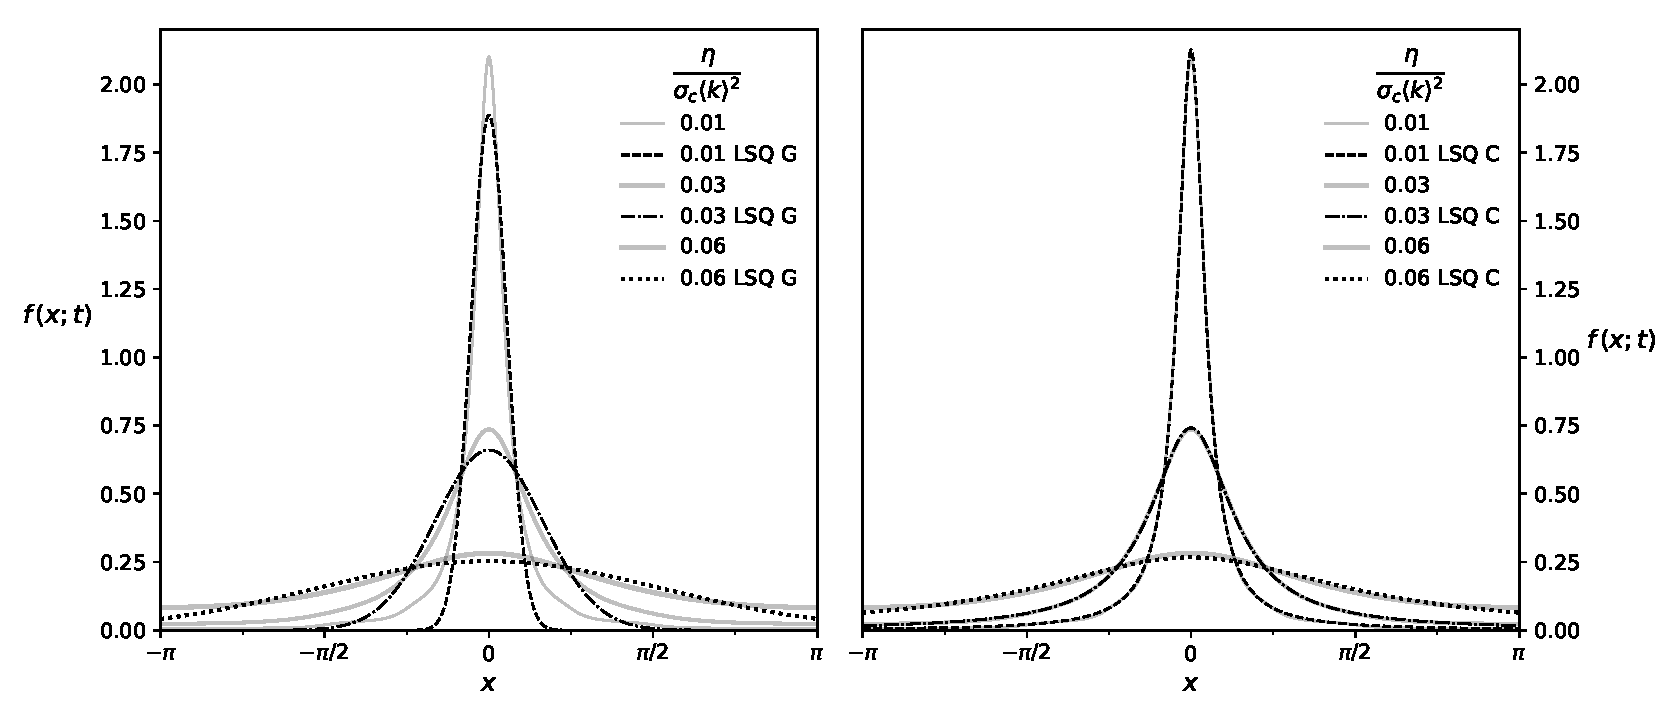
\includegraphics[width=1.2\linewidth]{figures/cont_mean_field_G_C_LSQ_BW}}%
	\caption{(soft curves) The final state distribution function $f(x,M\Delta t)$ for $M=3\cdot 10^5$, for various values of $\frac{\eta}{\sigma_c\langle k \rangle^2}$. (dashed/dotted curves, left) Least squares fits of the Gaussian distribution \cref{eq:gaussian_fit} to the final state distributions. (dashed,dotted curves, right) Least squares fits of the Cauchy distribution \cref{eq:cauchy_fit} to the final state distribution. The fit parameters and goodness of fit can be found in \cref{tab:fit_param_G_C_mean_field}. Legend entries are ordered from narrow to wide distributions.}	
	%		Model: Gaussian1D
	%		Inputs: ('x',)
	%		Outputs: ('y',)
	%		Model set size: 1
	%		Parameters:
	%		amplitude              mean               stddev      
	%		------------------ -------------------- ------------------
	%		1.8869199340983431 0.003931905699130531 0.1710214168889275 r^2 =  0.9702645006971661
	%		Model: Gaussian1D
	%		Inputs: ('x',)
	%		Outputs: ('y',)
	%		Model set size: 1
	%		Parameters:
	%		amplitude               mean               stddev      
	%		------------------ --------------------- ------------------
	%		0.6602437702220101 0.0039319056828550645 0.5157928158887003 r^2 =  0.9590595022517387
	%		Model: Gaussian1D
	%		Inputs: ('x',)
	%		Outputs: ('y',)
	%		Model set size: 1
	%		Parameters:
	%		amplitude              mean               stddev      
	%		------------------- -------------------- ------------------
	%		0.25310965580063377 0.003443017140767288 1.6525862408185896 r^2 =  0.9152246613834332
	%		Model: Lorentz1D
	%		Inputs: ('x',)
	%		Outputs: ('y',)
	%		Model set size: 1
	%		Parameters:
	%		amplitude             x_0                 fwhm       
	%		----------------- -------------------- ------------------
	%		2.126350006940973 0.003931891310500699 0.3127311371479785 r^2 =  0.9998347150194508
	%		Model: Lorentz1D
	%		Inputs: ('x',)
	%		Outputs: ('y',)
	%		Model set size: 1
	%		Parameters:
	%		amplitude              x_0                 fwhm       
	%		------------------ -------------------- ------------------
	%		0.7411141536424105 0.003928147410212121 0.9497871980512957 r^2 =  0.9998021024587377
	%		Model: Lorentz1D
	%		Inputs: ('x',)
	%		Outputs: ('y',)
	%		Model set size: 1
	%		Parameters:
	%		amplitude              x_0                 fwhm       
	%		------------------ -------------------- ------------------
	%		0.2669586944545997 0.003536080789641112 3.5380590656994206 r^2 =  0.981634500857006
	\label{fig:cont_mean_field_G_C_LSQ}
\end{figure}
\begin{table}[tbp]
	\caption{(a) Parameters $A$, $\sigma_f^2$ for the least squares Gaussian fits in the left graph of \cref{fig:cont_mean_field_G_C_LSQ}.  For all fits $\mu_f < 10^{-6}$. (b) Parameters $A$, $\gamma$ for the least squares Cauchy distribution fits in the right graph of \cref{fig:cont_mean_field_G_C_LSQ}, where $\gamma$ is scale parameter of the distribution. For all fits the location parameter $x_0 < 10^{-4}$. The goodness of fit $R^2$ and the area under the curve are denoted in the last two columns.}
	\label{tab:fit_param_G_C_mean_field}
	\begin{subtable}{.475\linewidth}
		\centering
		\caption{}
		\begin{tabular}{l|llll}
			$\frac{\eta}{\sigma_c\langle k \rangle^2}$ & $A$                        & $\sigma_f^2$               & $R^2$ & $\int\limits_{-\pi}^\pi dx\ f(x)$  \\ \hline
			$0.01$                      & 1.89                       & 0.0292                  & 0.9703 &	0.808\\
			$0.03$                      & 0.660                      & 0.266                   & 0.9591 &	0.852\\ 
			$0.06$                      & 0.253         			 & 2.73					   & 0.9152 &	0.987\\
		\end{tabular}
	\end{subtable}%
	\hfill
	\begin{subtable}{.475\linewidth}
		\centering
		\caption{}
		\begin{tabular}{l|llll}
			$\frac{\eta}{\sigma_c\langle k \rangle^2}$ & $A$    & $\gamma$   & $R^2$ &	$\int\limits_{-\pi}^\pi dx\ f(x)$   \\ \hline
			$0.01$                      & 2.12   & 0.1564 & 0.9998 & 1.01	\\
			$0.03$                      & 0.741  & 0.4750 & 0.9998 & 0.999	\\
			$0.06$                      & 0.267  & 1.769  & 0.9816 & 0.999	
		\end{tabular}
	\end{subtable}%
\end{table}

On the left-hand side of \cref{fig:cont_mean_field_G_C_LSQ}, we can clearly see that a Gaussian distribution does not fit the final state distribution well. For the sharpest peak, the fit is good anywhere where the distribution has a high slope, but the fit does not reach the peak value, nor is it high enough for $x$-values far from $x=0$. Hence, the area under the fitted distribution is less than 1, making it unfeasible. For wider distributions, the $R^2$ value increases, meaning that the fit quality is higher. But in these cases the maximum and minimum values are estimated too low. An analytic substitution of \cref{eq:gaussian_fit} in \cref{eq:cont_swarming_complete} using Maple 2018 verifies that a Gaussian is no steady state solution\footnote{We made an even extension of \cref{eq:gaussian_fit} at $x=-\pi$ and $x=\pi$ before substitution, to make sure the integrals are properly defined.}.

The right-hand side of \cref{fig:cont_mean_field_G_C_LSQ} shows the least squares fits of Cauchy distribution to the final state distributions. These curves seem to be a much better fit than the Gaussian distributions, an observation which can also be made quantitative by the goodness of fit $R^2$ in \cref{tab:fit_param_G_C_mean_field}. Furthermore, the area under the curves is very close to $1$, corresponding with feasible state distributions. However, a closer look at the distribution corresponding to $\frac{\eta}{\sigma_c\langle k \rangle^2} = 0.06$ shows that a Cauchy distribution might not be the perfect analytic description of the stationary state distribution.  Substitution of \cref{eq:cauchy_fit} confirms this last observation\footnote{Again an even extension was made to \cref{eq:cauchy_fit} before substitution.}. 

It should be remarked that both Gaussian and Cauchy distributions yield the constant value $\frac{1}{2\pi}$ if we take the limit of respectively the variance or the half-width at half-maximum to infinity before renormalising on $[-\pi,\pi)$. This corresponds to the distribution of the disordered system. Moreover, they converge to a Dirac distribution if we take the same limit to zero, corresponding to a perfectly ordered system. Therefore it might be worthwhile for further research to check whether all steady-state distributions, i.e. either disordered and ordered, can be described by another bell-shaped distribution with the same properties, where one allows for taking the limit cases $\sigma_f^2 \to \infty$ and $\sigma_f^2 \to 0$ or $\gamma \to \infty$ and $\gamma \to 0$. 

\section{Moment closure approximation on swarming systems}
The same rules and assumptions with which we defined a swarming system in \cref{section:applying_network_to_swarming} will be applied to the moment closure approximation of continuous state adaptive networks in this section. Afterwards, analysis and discussion of the results will follow. 

The system consisting of two coupled non-linear partial integro-differential equations which make an adaptive network model two dimensional collective motion in a swarm is written as 
\raggedbottom
\begin{subequations}
	\label{eq:cont_swarming_complete}\small
	\begin{adjustwidth}{-.5in}{-.5in} 
		\begin{align}
		\frac{\partial f(x;t)}{\partial t} =\ &
		\eta \left( \frac{1}{2\pi} - f(x;t) \right) \\
		& + \sigma_c\int\limits_{-\pi}^\pi dz \int\limits_0^{\pi/2} d \xi  \
		\Bigg[ 
		\frac{l(x-\xi ,z;t)\ l(z,x+\xi ;t)}{f(z;t)} - \frac{l(z-\xi ,x;t)\ l(x,z+\xi ;t)}{f(x;t)} 
		\Bigg] \nonumber  \\[15pt]
		\frac{\partial l(x,y;t)}{\partial t} = &
		\int\limits_{-\pi}^\pi dz \
		\Bigg{\{ }
		\frac{\eta}{2\pi} \left( l(x,z;t) + l(z,y;t) \right)  \\
		& \phantom{\int\limits_{-\pi}^\pi dz\ \sum}
		+\sigma_c \frac{l(y,z;t)\ l(z,-y+2x;t)}{f(z;t)}
		+\sigma_c \frac{l(x,z;t)\ l(z,-x+2y;t)}{f(z;t)} \nonumber\\
		& \phantom{\int\limits_{-\pi}^\pi dz\ \sum}
		-\sigma_c \frac{l(y,x;t)\ l(x,z;t)}{f(x;t)} 	 
		-\sigma_c \frac{l(x,y;t)\ l(y,z;t)}{f(y;t)} \nonumber \\
		& \phantom{\int\limits_{-\pi}^\pi dz\ \sum}
		+ \sigma_c\int\limits_0^{\pi/2} d \xi \    
		\Bigg[  
		\frac{l(y,z;t)\ l(z, x-\xi;t)\ l(z, x+\xi;t)}{f(z;t)^2}  + 
		\frac{l(x,z;t)\ l(z, y-\xi;t)\ l(z,y+\xi ;t)}{f(z;t)^2} \nonumber\\ 
		& \phantom{\int\limits_{-\pi}^\pi dz\ \sum \sigma_c\int\limits_0^{\pi/2} \ d \xi \sum }
		- \frac{l(y,x;t)\ l(x, z-\xi;t)\ l(x,z+\xi ;t)}{f(x;t)^2} - 
		\frac{l(x,y;t)\ l(y, z-\xi ;t)\ l(y, z+\xi ;t)}{f(y;t)^2} 
		\Bigg]	 \
		\Bigg{ \} } \nonumber\\
		&+ \alpha\ f(x;t)\ f(y;t) - 
		(2\eta+\beta)\ l(x,y;t). \nonumber
		\end{align}
	\end{adjustwidth}
\end{subequations}

\normalsize Here we assumed the discrete closure relation from \cite{Chen2016} to be applicable in the continuous state case. 
\normalfont

\subsection{Discretisation}
Similar to the mean field approximation, we will look for numerical solutions to the system of equations (\ref{eq:cont_swarming_complete}). A first step into solving this system numerically is discretising the time and state sets and transforming the partial integro-differential equations into partial \textit{difference} equations. This discretisation will be conducted in a similar manner compared to the mean field approximation model. That is, the continuous time $t = [0, T_{\text{max}}]$ at which the network evolution is considered will be partitioned into $M$ intervals of length $\Delta t$, such that the discrete time set is of the form 
\[ t_d= \{0, \Delta t, 2 \Delta t, ... , (\tau-1) \Delta t,  \tau\Delta t, ..., T_{\text{max}} - \Delta t, T_{\text{max}}  \}, \]
such that $M \Delta t = T_{\text{max}}$ and $\tau$ is the discrete time index. Furthermore, the state set $\Omega$ is partitioned into $N$ intervals of length $\Delta \omega$, such that $\Omega = [-\pi,\pi)$ is transformed into 
\[\Omega_d = \{-\pi, -\pi+\Delta\omega,...,-\pi+ (p-1) \Delta\omega, -\pi+ p \Delta\omega, ... \pi-\Delta\omega, \pi \}, \]
in which $N \Delta \omega = 2\pi$ and $p$ is the discrete state index.

To keep things clear, we will use the following shorthand notation in the discretisation of the density functions $f$ and $l$ on the discrete state-time-grid. 

\begin{equation}
f_{p}^{\tau } = f(-\pi+p\Delta \omega; \tau \Delta t) \qquad l_{p,q}^{\tau }=l(-\pi+p\Delta\omega,-\pi+q\Delta\omega;\tau \Delta t).
\end{equation}
The grid on which $f_{p}^{\tau}$ is defined is visualised in \cref{fig:grid_pde}. For $l_{p,q}^\tau$ we have something similar, but then on a three-dimensional grid. Again the forward difference method is applied to discretise the partial derivatives, such that for the state distribution $f$ we have \cref{eq:forward_difference_f}, whilst for the link distribution $l$ we have
\begin{equation}
\frac{\partial}{\partial t}\ l(x,y;t) \approx \frac{l(x,y;t+\Delta t) - l(x,y;t)}{\Delta t} = \frac{l_{p,q}^{\tau+1} - l_{p,q}^{\tau}}{\Delta t},
\end{equation}
for $x = -\pi + p \Delta \omega $ and $y = -\pi + q \Delta \omega $. Once again, we take the left Riemann sums as discretisation for the integrals, just as in \cref{eq:left_riemann}. Taking everything together, the system of partial difference equations describing a continuous state adaptive network becomes

\begin{subequations}\label{eq:cont_swarming_complete_forward_Euler}
	\begin{alignat}{2}
	\frac{f_{p}^{\tau +1} - f_{p}^{\tau }}{\Delta t} = & 
	\ \eta \left(\frac{1}{2\pi} - f_{p}^{\tau } \right) + 
	\sigma_c\ \Delta\omega^2 \sum\limits_{j=0}^{N-1}\sum\limits_{i=0}^{\frac{N}{4}-1}  
	\Bigg(
	\frac{l_{p-i,j}^{\tau }\  l_{j,p+i}^{\tau }}{f_{j}^{\tau }} - 
	\frac{l_{j-i,p}^{\tau }\ l_{p,j+i}^{\tau }}{f_{p}^{\tau }} 
	\Bigg)\\[15pt]
	\frac{l_{p,q}^{\tau +1} - l_{p,q}^{\tau }}{\Delta t} = & 
	\sum\limits_{j=0}^{N-1} \Delta \omega 
	\Bigg[
	\frac{\eta}{2\pi} \left( l_{p,j}^{\tau } + l_{j,q}^{\tau }\right) \\
	& \phantom{\sum\limits_{j=0}^{N-1} \Delta \omega\sum\limits_{j=0}^{N-1} } 
	+ \sigma_c \frac{l_{q,j}^{\tau}\ l_{j,-q+2p}^{ \tau}}{f_{j}^{\tau}}
	+ \sigma_c \frac{l_{p,j}^{\tau}\ l_{j,-p+2q}^{ \tau}}{f_{j}^{\tau}}
	- \sigma_c \frac{l_{q,p}^{\tau }\ l_{p,j}^{\tau }}{f_{p}^{\tau }} 
	- \sigma_c \frac{l_{p,q}^{\tau }\ l_{q,j}^{\tau }}{f_{q}^{\tau }} \nonumber  \\
	& \phantom{\sum\limits_{j=0}^{N-1} \Delta \omega\sum\limits_{j=0}^{N-1} } 
	+ \sigma_c\ \Delta \omega \sum\limits_{i=0}^{\frac{N}{4}-1}  
	\Bigg(
	\frac{l_{q,j}^{\tau }\ l_{j, p-i}^{\tau }\ l_{j, p+i}^{\tau }}{(f_{j}^{\tau })^2}
	+ \frac{l_{p,j}^{\tau }\ l_{j, q-i}^{\tau }\ l_{j, q+i}^{\tau }}{(f_{j}^{\tau })^2}	\nonumber \\
	& \phantom{\sum\limits_{j=0}^{N-1}\sum\limits_{j=0}^{N-1} \Delta \omega \sigma_c\sum\limits_{i=0}^{\frac{N}{4}-1} \Delta \omega\sum }
	- \frac{l_{q,p}^{\tau }\ l_{p, j-i}^{\tau }\ l_{p,j+i}^{\tau }}{(f_{p}^{\tau })^2}
	- \frac{l_{p,q}^{\tau }\ l_{q, j-i}^{\tau }\ l_{q,j+i}^{\tau }}{(f_{q}^{\tau })^2}
	\Bigg)
	\Bigg] \nonumber \\
	&+ \alpha\ f_{p}^{\tau }\ f_{q}^{\tau }
	- (2\eta+\beta)\ l_{p,q}^{\tau }.\nonumber
	\end{alignat}
\end{subequations}
This system of equations can be rewritten as a forward Euler scheme, allowing for numerically computing the time evolution in any appropriate computing language, given feasible initial conditions.



\subsection{Results and discussion}
The forward Euler scheme of \cref{eq:cont_swarming_complete_forward_Euler} was implemented in Python. The input parameters of the script are the system parameters $\eta$, $\sigma_c$, $\alpha$ and $\beta$, step size $\Delta t = \frac{1}{400}$, and grid spacing $\Delta \omega = \frac{2\pi}{23}$. To generate results the system was solved for five different initial conditions (before normalisation): $\mathcal{N}(0,5)$, $\mathcal{N}(0,1)$ and  $\frac{1}{2\pi}+a\, \cos(x)$, for $a\in\left\lbrace\frac{1}{10}, \frac{1}{40}, \frac{1}{400}\right\rbrace$.  $\mathcal{N}(\mu,\sigma_f^2)$ indicates the normal distribution with mean $\mu$ and variance $\sigma_f^2$.

The link distribution function is initialised as 2-dimensional standard normal distribution. That is 
\begin{equation}\label{eq:IC_link}
	l(x,y;0)=\frac{1}{2\pi} \exp\left(-\frac{1}{2} \left(x^2+y^2\right) \right).
\end{equation} 
Similar to the discrete state models and the continuous state mean field approximation, the solution converges to a disordered solution if the ratio of the noise rate $\eta$ to the three-body interaction rate $\sigma_c$ is high enough. For this case, the state distribution function $f(x;t)$ is plotted for two different initial conditions in \cref{fig:cont_closure_state_t_disordered_IC1_IC6_s4}. If this rate is low enough the system converges to an ordered solution, which is visualised in \cref{fig:cont_closure_invertingbehaviour_IC2_IC3_s7} for two different initial conditions. For most initial conditions, the time evolution is similar to the graph on the left-hand side and is as expected. The graph on the right-hand side shows a phenomenon which was not encountered before; the highest density states at $\tau=0$ converge to a density of 0, whilst the lower density states end up dominating the system. This behaviour is most likely caused by the discretisation of the system. For example, if in the first time step the change in the peak value of the state distribution is bigger than $-2a=-\frac{1}{200}$ the distribution at $\tau=1$ will be inverted. If the change in consecutive time steps is smaller, then convergence to an inverted ordered state can be explained. One can check if this is really the case by testing if similar results are obtained when smaller time steps and more grid points in $\Omega$ are taken. 

\begin{figure}[tbp]
	\centering
	\makebox[\textwidth][c]{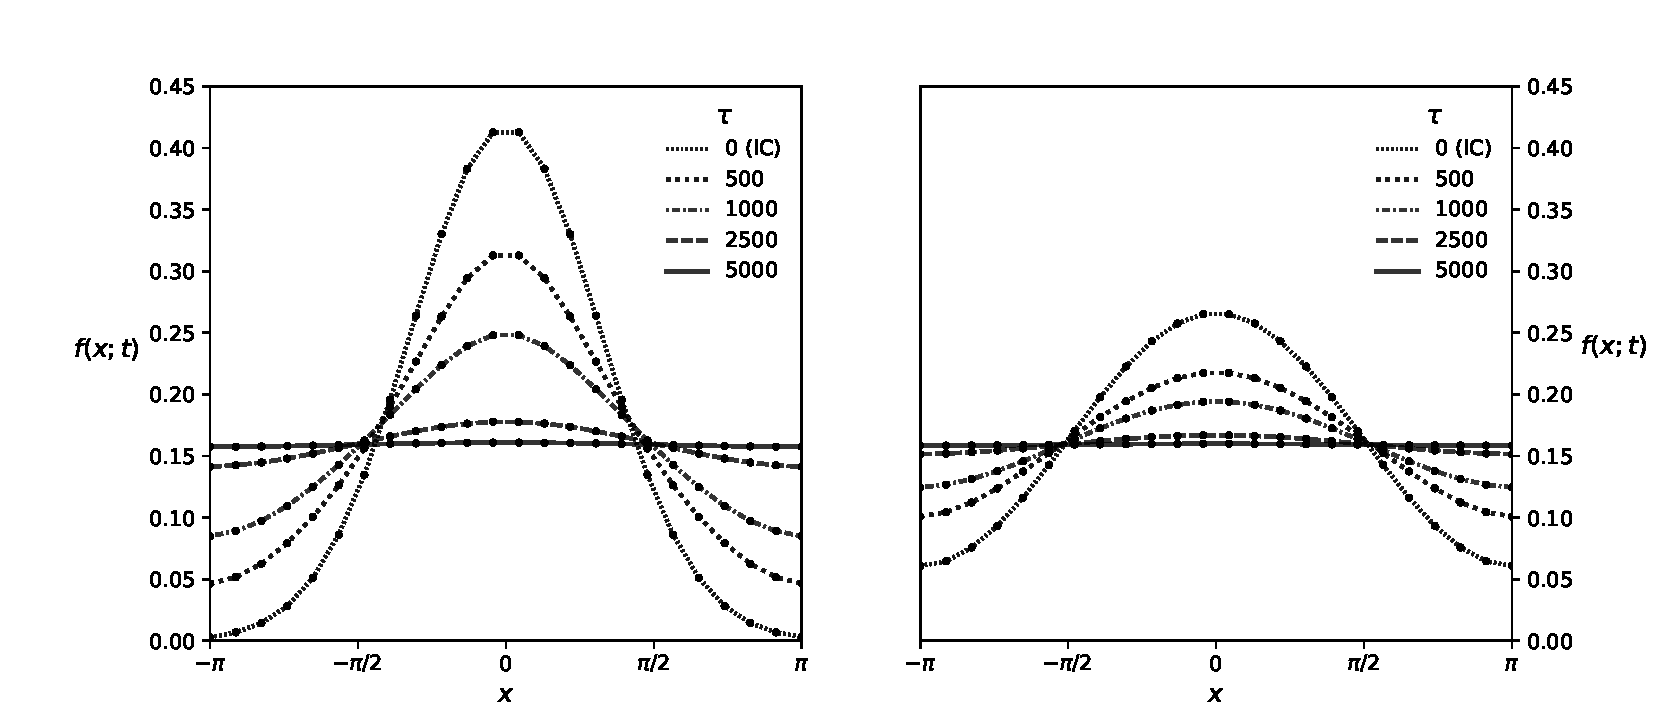
\includegraphics[width=1.2\linewidth]{figures/cont_closure_state_t_disordered_IC1_IC6_s4}}%
	\caption{The state distribution function $f(x;\tau \Delta t)$ for various values of $\tau$. The system parameters are $\eta=1$, $\sigma_c =4$, $\alpha=0.1$, $\beta=0.1$. The initial condition (IC) was taken as $f(x;0)~=~\mathcal{N}(0,1)$ (left) and $f(x;0)~=~\frac{1}{2\pi}+\frac{1}{10} \cos(x)$ (right). Both solutions converge to the disordered stationary solution. Grid points are indicated with dots.}
	\label{fig:cont_closure_state_t_disordered_IC1_IC6_s4}
\end{figure}

\begin{figure}[tbp]
	\centering
	\makebox[\textwidth][c]{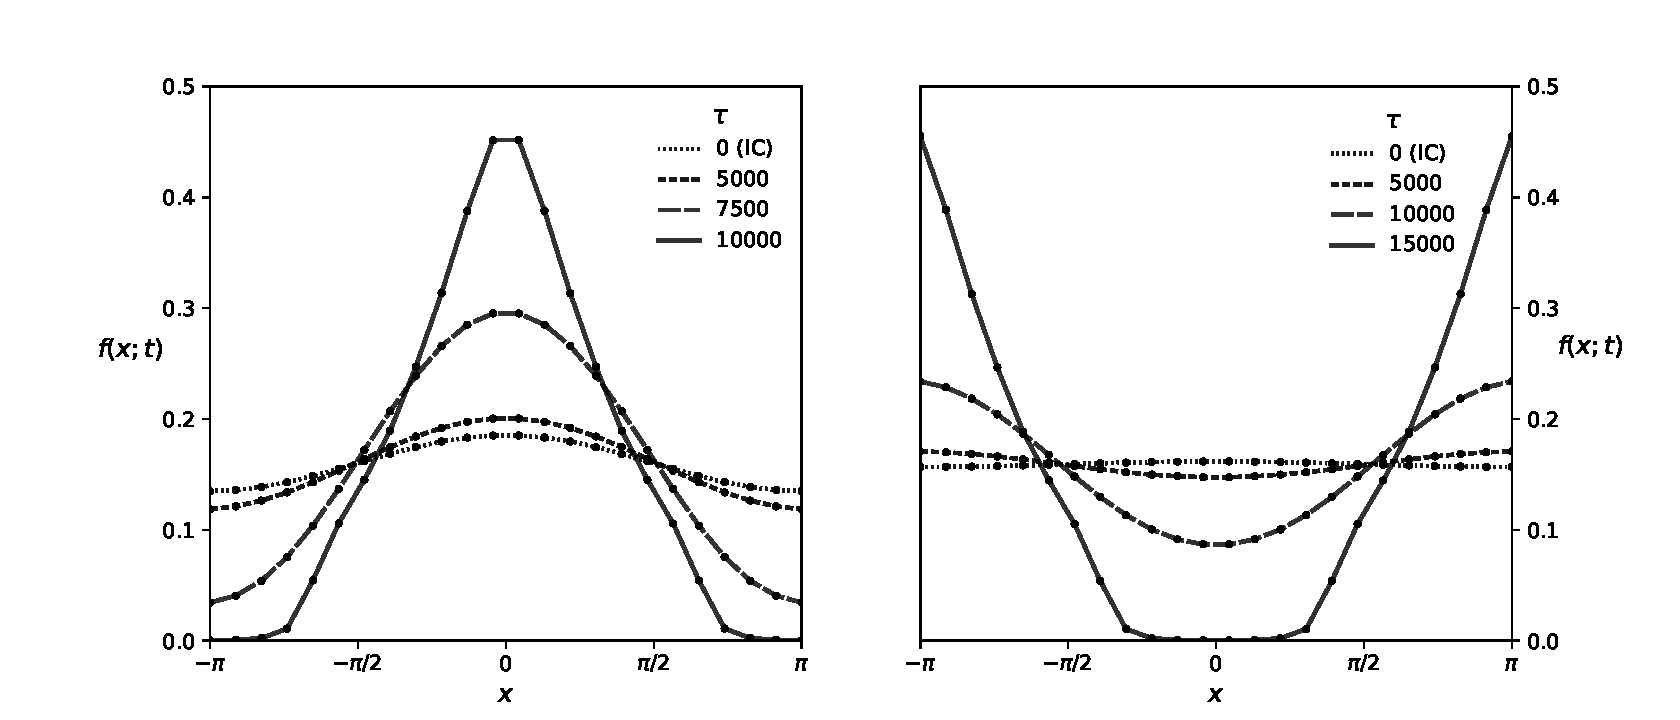
\includegraphics[width=1.2\linewidth]{figures/cont_closure_invertingbehaviour_IC2_IC3_s7}}%
	\caption{The state distribution function $f(x;\tau \Delta t)$ for various values of $\tau$. The system parameters are $\eta=1$, $\sigma_c =7$, $\alpha=0.1$, $\beta=0.1$. The initial condition (IC) was taken as $f(x;0)~=~\frac{1}{2\pi}+\frac{1}{40} \cos(x)$ (left) and $f(x;0)~=~\frac{1}{2\pi}+\frac{1}{400} \cos(x)$ (right). Both solutions converge to an ordered stationary solution. Grid points are indicated with dots.}
	\label{fig:cont_closure_invertingbehaviour_IC2_IC3_s7}
\end{figure}

As with the mean field approximation, we use the variance $\sigma_f^2$ of the state distribution as a measure for the amount of order in the system. In \cref{fig:cont_closure_variance_vs_sigma} the variance of the final distribution $f(x;M\Delta t)$ after $M=2\cdot 10^4$ time steps was plotted as function the ratio of system parameters $\frac{\eta}{\sigma_c}$ for all five initial conditions. For relatively high noise ratios $\left(\frac{\eta}{\sigma_c} \ge \frac{1}{5.2}\right)$ the system converges to the disordered solution and therefore $\sigma_f^2=\frac{\pi^2}{3}$. For a relatively low ratio $\left(\frac{\eta}{\sigma_c} \le \frac{1}{6.6}\right)$ the system converges to a disordered solution with nearly constant variance for all initial conditions. Note that this was not the case in the mean field approximation, where the final state distribution variance was depending on the system parameters by a square root relation. For $\frac{1}{6.6}\le\frac{\eta}{\sigma_c}\le\frac{1}{5.2}$ there is a bistable region, where the exact stationary solution depends on the initial condition. This may be a sign that the system has a subcritical (pitchfork) bifurcation at either of the two ends of the bistable region in combination with a saddle-node bifurcation at the other end. \Cref{fig:cont_closure_saddle_IC1_s5331} shows another sign of the presence of these bifurcations. The system initialised as standard normal distribution seems to converge to the disordered solution $f(x;t) = \frac{1}{2\pi}$ at first sight. However, after $\tau=7000$, the distribution stops flattening out and it starts converging to an ordered stationary solution, which is indicated by the star in \cref{fig:cont_closure_variance_vs_sigma}. This is an indication that the disordered solution forms a saddle-node for these parameters and the distribution gets close to the saddle-node in phase space before converging to its stable stationary solution. 
Note that we cannot determine the exact system parameters for which this bifurcation occurs with current solutions for only five different initial conditions. Further research is needed to determine the exact location and details of this bifurcation. Moreover, the exact reason why the \textit{ordered} state distribution has an almost constant variance for various values of the system parameters could be a subject of future research. 

\begin{figure}[tbp]
	\centering
	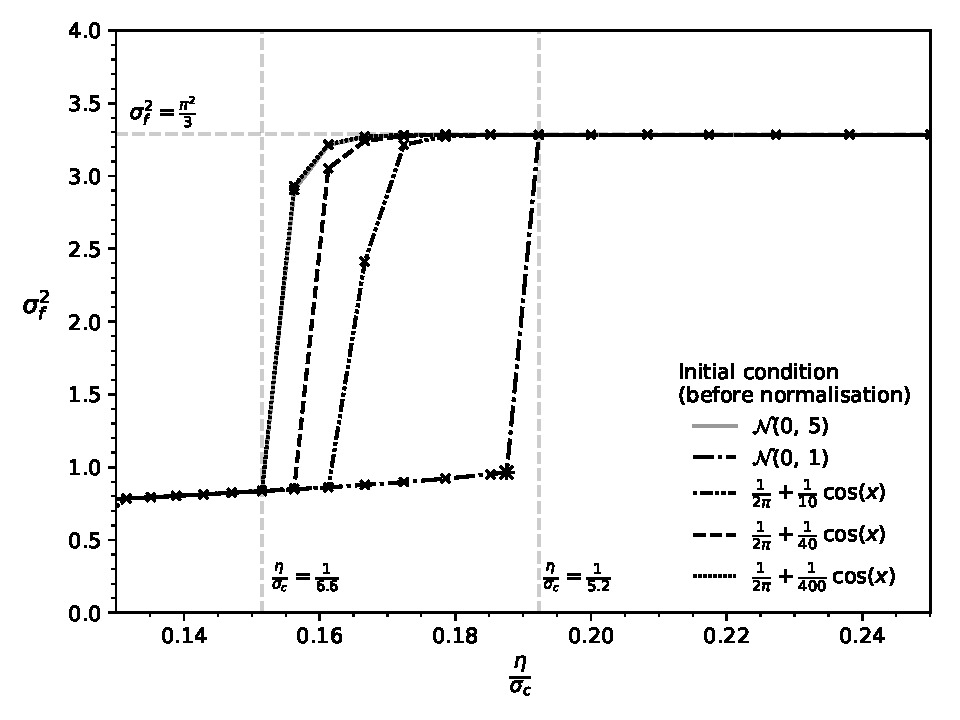
\includegraphics[width=0.7\linewidth]{figures/cont_closure_variance_vs_etaoversigma}%
	\caption{Variance $\sigma_f^2$ of the stationary state of the state distribution $f(x;t)$ as function of the ratio of system parameters $\frac{\eta}{\sigma_c}$ for various initial conditions. The system parameters were taken as $\eta=1$, $\alpha=0.1$,  $\beta=0.1$, $\sigma_c$ was varied. For $\frac{\eta}{\sigma_c}\ge\frac{1}{5.2}$ all distributions converged to the disordered stationary state solution, while for $\frac{\eta}{\sigma_c}\le\frac{1}{6.6}$ all distributions converged to an ordered solution. For $\frac{1}{6.6}\le\frac{\eta}{\sigma_c}\le\frac{1}{5.2}$ the stationary state solution depends on the chosen initial condition. The star indicates $\frac{\eta}{\sigma_c} = \frac{1}{5.331}$, for which the time evolution is plotted in \cref{fig:cont_closure_saddle_IC1_s5331}.}
	\label{fig:cont_closure_variance_vs_sigma}
\end{figure}

\begin{figure}[tbp]
	\centering
	\makebox[\textwidth][c]{\quad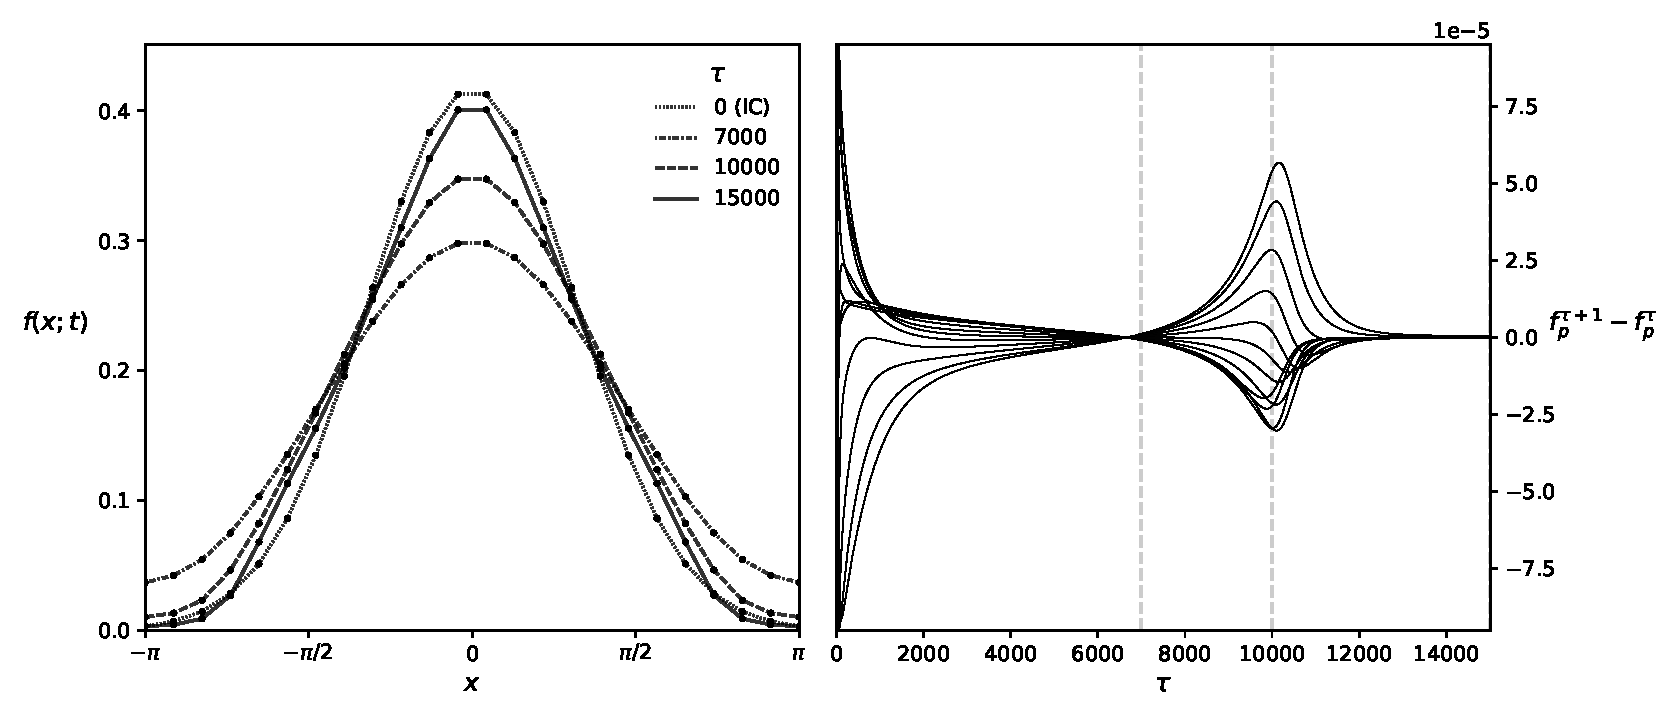
\includegraphics[width=1.2\linewidth]{figures/cont_closure_saddle_IC1_s5331}}%
	\caption{(left) The state distribution function $f(x;\tau \Delta t)$ for various values of $\tau$. The system parameters are $\eta=1$, $\sigma_c =5.331$, $\alpha=0.1$, $\beta=0.1$. The initial condition (IC) was taken as $f(x;0)~=~\mathcal{N}(0,1)$. Grid points are indicated with dots. (right) The difference $f_p^{\tau+1}-f_p^\tau$ between two consecutive state distribution functions for $p\in [0,...,11]$ versus the discrete time index $\tau$. Similar curves are obtained for $p\in [12,...,23]$ since the distribution is symmetric for all $\tau$. The distribution converged to a disordered solution, despite of the fact that it flattens out in the first 7000 time steps. }
	\label{fig:cont_closure_saddle_IC1_s5331}
\end{figure}


Some more remarks should be added about the (implementation of) the current numerical method which solves the system. More recommendations for future research will naturally follow. The most important limitation of the current script occurs when the ratio of the noise rate to the three-body interaction rate is taken too low $\left(\frac{\eta}{\sigma_c} \lesssim \frac{1}{8}\right)$. Then for some $\tau$, the distribution will get too narrow to be represented properly by $24$ grid points. That is, there is a time step after which the obtained curve is not smooth enough, introducing unacceptable numerical errors in consecutive time steps. Moreover, the smallest values of the state distribution function get so small, that extra numerical errors are obtained when these numbers get multiplied or divided by each other and by other numbers. Multiple things have been implemented to reduce these errors, amongst others calculating with 128-bit floating-point numbers, preventing division by small numbers, reducing the time step and implementing an implicit Euler backward integration method. These are however no permanent fixes for the problem. To resolve this issue permanently, one could find a way to increase the resolution of the state set $\Omega$ to more than $24$ grid points. This requires significant optimisation of the current computation time first. Moreover, one could look at alternative numerical methods to find stationary solutions, such as Newton-Raphson methods for systems of differential equations. The latter being rather a workaround than a solution since it does not allow for time evolution, but only for finding stationary solutions. If one finds higher resolution stationary state distributions, then it will be worthwhile to check whether the Cauchy distribution (or another bell-shaped distribution) can be the true analytic stationary solution to the system using more sophisticated PDE techniques.

Furthermore, future research could focus more on the link distribution function $l(x,y;t)$. That is, finding its steady state distributions, looking for bifurcations, investigating the influence of a different initial condition than \cref{eq:IC_link} and exploring the effect of different values for $\alpha$ and $\beta$. One could also do more research into how more sophisticated initial distributions evolve. This might be done by deriving and analysing a PDE for the change in the mean of the distribution
\begin{equation}
\frac{d}{dt} \langle x \rangle = \frac{\partial}{\partial t} \int\limits_\Omega dx\ x\ f(x;t)
\end{equation}
and by deriving and analysing the a PDE for change of the second moment
\begin{equation}
\frac{d}{dt} \langle x^2 \rangle = \frac{\partial}{\partial t} \int\limits_\Omega dx\ x^2\ f(x;t),	
\end{equation}
which is a measure for the amount of order in the system.

With all this information, the comparison between adaptive network models, other models for swarming systems and real life swarming systems can be made. Subsequently, one can find out how accurate adaptive network models are and where improvement might be needed. For example, it may be that adding other types of dynamics yields more accurate and realistic predictions. Finally, it will be interesting whether there are cases in which adaptive network models are better or more convenient than the current models.



